\documentclass[a0, portrait]{a0poster}
%%%Load packages
\usepackage{multicol} 			%3-column layout
\usepackage[left=1.5cm,right=1.5cm,bottom=0cm,top=0cm]{geometry}			%Reset margins
%\usepackage{fontspec} % For loading fonts
%\setmainfont[SmallCapsFont = Fontin SmallCaps, Ligatures=TeX]{Fontin} % Main document font
\usepackage[scaled=1]{helvet}
\usepackage[x11names]{xcolor}				%Needed for colour boxes & coloured text
\usepackage{graphicx}%%%Define colours and lengths
\usepackage[export]{adjustbox}
\usepackage{authblk}
    \usepackage{amsmath} % Equations
    \usepackage{amssymb} % Equations
\usepackage{bbm} %mathbbm
\usepackage{anyfontsize}
\usepackage{array, booktabs}
\usepackage[utf8]{inputenc}
\usepackage{tcolorbox}
\usepackage{cleveref}
\usepackage[hidelinks, linktoc=all, russian]{hyperref}
\usepackage{capt-of}
\usepackage[font=small,labelfont=bf]{caption}
\usepackage{subcaption}
\captionsetup[subfigure]{justification=centering, labelformat=parens}
\captionsetup[figure]{justification=centering}

\definecolor{headingcol}{rgb}{0.4, 0.57, 0.83}			%Colour of main title
\definecolor{titlecol2}{HTML}{CC181E}			%Colour of main title

\definecolor{titlecol}{rgb}{0.3, 0.47, 0.73}			%Colour of main title
\definecolor{boxcol}{rgb}{0.7,0.2,0.2}		%Edge-colour of box and top banner
\fboxsep=1cm							%Padding between box and text
\setlength{\columnsep}{2cm}				%Set spacing between columns
\renewcommand{\familydefault}{\sfdefault}	%Set main text to sans-serif


\newenvironment{frshaded}{%
\def\FrameCommand{\fboxrule=\FrameRule\fboxsep=\FrameSep \fcolorbox{framecolor}{shadecolor}}%
\MakeFramed {\FrameRestore}}%
{\endMakeFramed}

\renewcommand{\figureautorefname}{Fig.}%
\renewcommand{\figurename}{Fig.}


\begin{document}

\begin{center}
\vspace*{-2cm}
\hspace*{-2cm}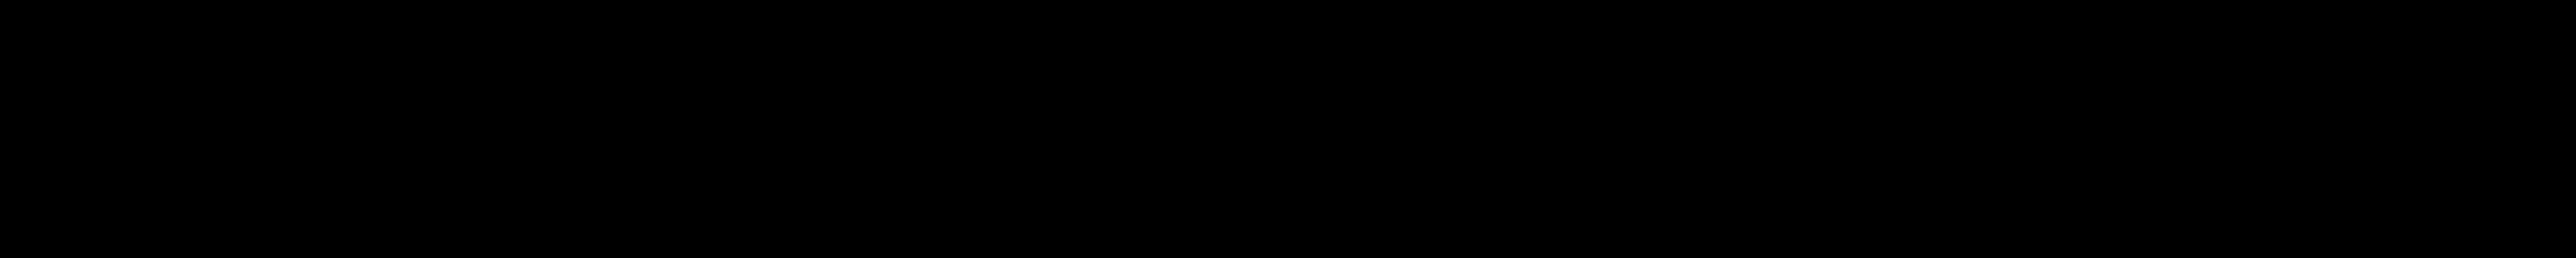
\includegraphics[width=1.2\textwidth]{Black_Landscape}
\end{center}


%%% Title
\begin{minipage}{0.65\textwidth}					
\vspace{-11cm}
\begin{tabular}[t]{l}
{\color{headingcol}\fontsize{68}{70}\selectfont Observing the non-analytic behaviour of a qubit-resonator system}\\
\\
{\hspace{1cm} \color{white}\Large Gleb Fedorov$^{1,2}$, Evgenii Glushkov$^{1,2}$ and Kirill Shulga$^{1,2,3}$}\\
\\
{\hspace{1.2cm}\color{white}\large $^1$\textit{Moscow Institute of Physics and Technology \hspace{1cm} $^2$Moscow Institute of Steel and Alloys \hspace{1cm} $^3$Russian Quantum Center}}
\end{tabular}
\end{minipage}
%%% Logos
\hspace{19cm}
\begin{minipage}{0.35\textwidth}
\vspace{-11cm}
\begin{tabular}{c c}

\includegraphics[height=0.035\textheight]{misislogo}\\

\includegraphics[height=0.0225\textheight]{miptlogo}
\end{tabular}
\end{minipage}


\vspace{-1.5cm}
\begin{multicols}{2}							%Use 3-column layout
%\raggedcolumns							%Don't stretch contents vertically

%%%Column1

\tcbset{colframe=titlecol, colback=white}
\begin{tcolorbox}[left=1cm, right=1cm, top=0.5cm, bottom=0.5cm, 
                  title={\Large Introduction}, bottomtitle=.5cm,toptitle=.5cm]
\begingroup
\setlength{\columnsep}{1cm}	
\begin{multicols}{2}
The performance of superconducting qubits has improved by several orders of magnitude in the past decade. The most successful and prominent studies\cite{bishop2009} in this field are all about circuit Quantum Electrodynamics (cQED) or so-called ``quantum optics on a chip''. In this work we've been trying to test if our sample was robust enough to reproduce quantitatively famous effects predicted by so-called ``Rabi model''.
\end{multicols}
\endgroup
\end{tcolorbox}

\tcbset{colframe=titlecol, colback=white}
\begin{tcolorbox}[left=1cm, right=1cm, top=0.5cm, bottom=0.5cm, 
                  title={\Large Flux qubit}, bottomtitle=.3cm, toptitle=.5cm
                  ]

In the experiment we've carried out the Flux qubit was used. Firstly suggested in 1999, this qubit consists of a superconducting loop, interrupted three times with three Josephson junctions as depicted on \autoref{fig:qubit}~(a),~(b).\\

\begin{minipage}{\textwidth}
\centering
\begin{tabular}{c@{\hspace{1.5cm}}c@{\hspace{1cm}}c}
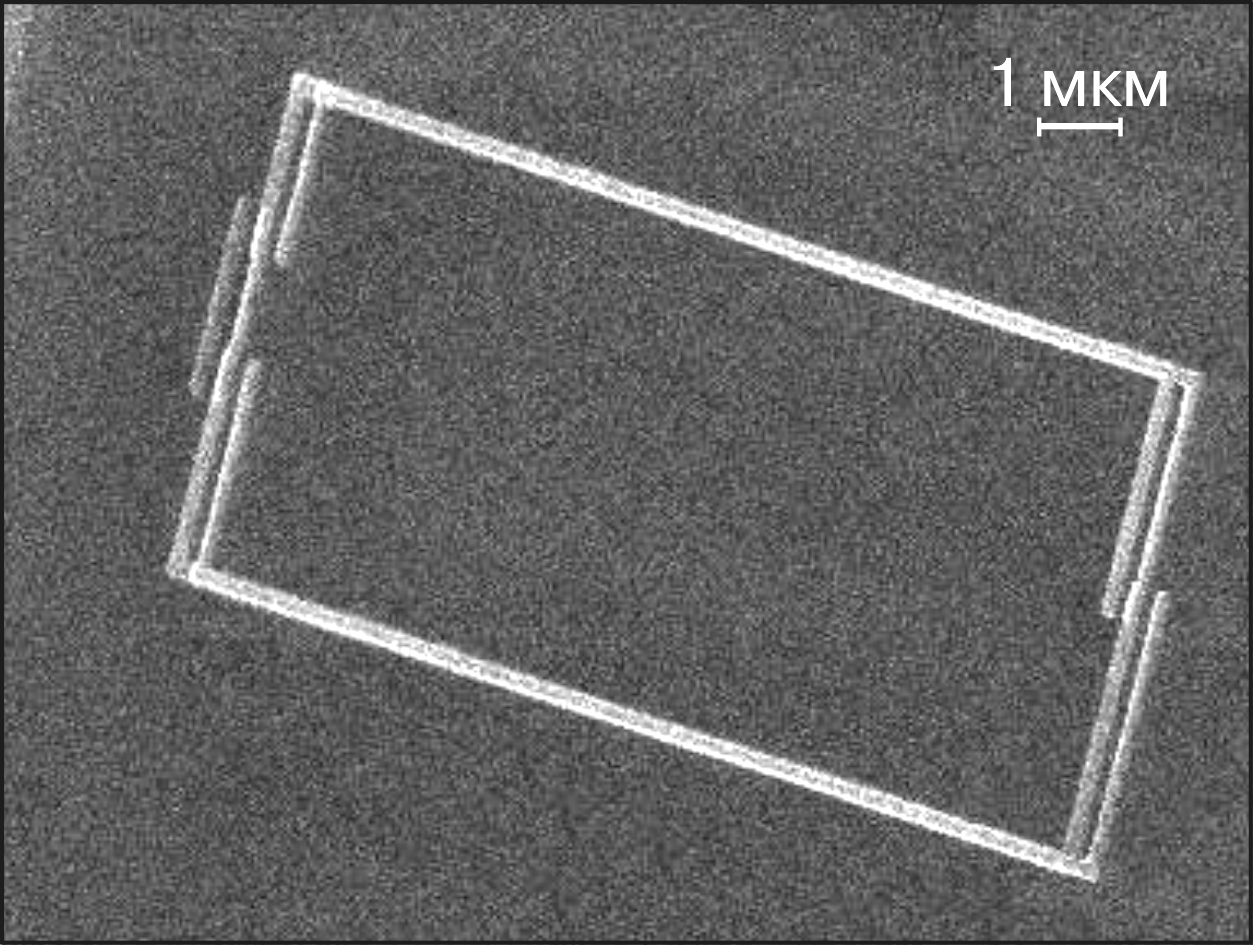
\includegraphics[valign=t, scale=0.25]{Pictures/qubit_photo} &
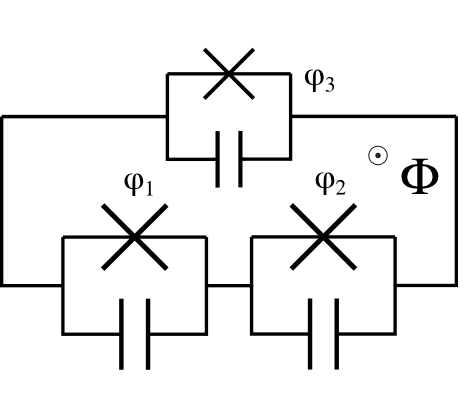
\includegraphics[valign=t, scale=1.4]{Pictures/qubit_clean} &
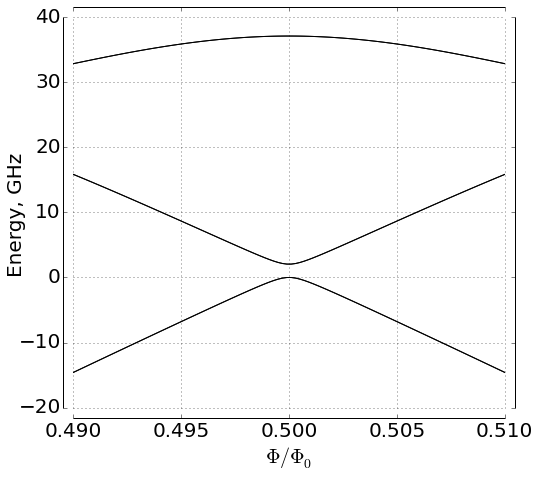
\includegraphics[valign=t, scale=0.55]{Pictures/qubit_3levels}\\
\parbox[bottom][2.5cm][t]{10cm}{\captionof{subfigure}{SEM micrograph of a three-junction Flux qubit}}\label{fig:qubit_a} &
\parbox[bottom][2.5cm][t]{10cm}{\captionof{subfigure}{RCSJ model of Flux qubit}} &
\parbox[bottom][2.5cm][t]{10cm}{\captionof{subfigure}{The three lowest energy bands}}\\
\end{tabular}
\end{minipage}

\begin{minipage}{\textwidth}
\centering
\captionof{figure}{Flux qubit, its theoretical model and numerically computed energy spectrum}
\label{fig:qubit}
\end{minipage}

RCSJ model of the Josephson junction and the quantization of flux allows to write down the Hamiltonian of the Flux qubit and solve it for eigenenergies and eigenstates. The first three of numerically calculated energy levels are presented on \autoref{fig:qubit}~(c). The difference $E_1 - E_0$ shows hyperbolic dependence on $\Phi$ (\autoref{fig:qubit_spectrum}).\\

\begin{minipage}{0.5\textwidth}
\centering
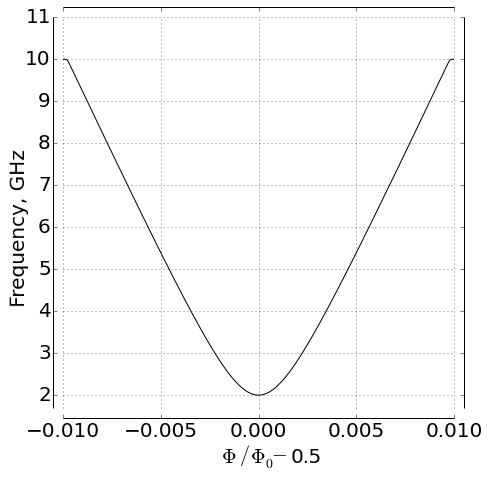
\includegraphics[height=12cm]{Pictures/spectrum_hyp}
\captionof{figure}{Flux qubit spectrum}
\label{fig:qubit_spectrum}
\end{minipage}
\begin{minipage}{0.5\textwidth}
Using the form of the qubit potential and the tight-binding model it is possible to extract the reduced two-level Hamiltonian, which is valid in the vicinity of the degeneracy point:
\begin{equation}
\mathcal{\hat H} = \frac{\varepsilon}{2}\,\hat \sigma_z + \frac{\Delta}{2}\,\hat \sigma_x,
\label{eq:red_ham}
\end{equation}
where $\varepsilon \propto \Phi-\Phi_0/2$ and $\Delta = const$ is responsible for the minimal splitting. From this we get the theoretical formula of the numerically obtained spectrum on \autoref{fig:qubit_spectrum}:
\begin{equation}
\Delta E = \hbar \omega_q = \sqrt{\varepsilon^2+\delta^2}.
%\label{eq:qub_spec}
\end{equation}
\end{minipage}\\
\end{tcolorbox}

\tcbset{colframe=titlecol}
\begin{tcolorbox}[left=1cm, right=1cm, top=0.5cm, bottom=0.5cm, 
                  title={\Large Sample design}, bottomtitle=.3cm,toptitle=.5cm
                  ]
\begin{minipage}{0.5\textwidth}
\centering
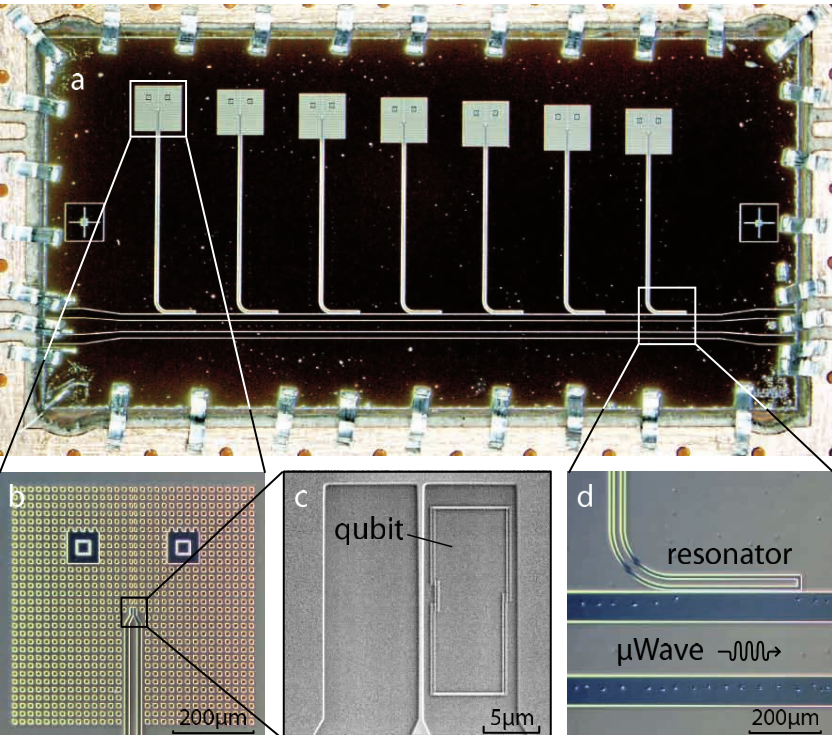
\includegraphics[height=13cm]{Pictures/marcus_chip}
\captionof{figure}{Seven qubit-resonator systems coupled to the transmission line}
\end{minipage}
\begin{minipage}{0.5\textwidth}
In the experiment we used a chip with seven different $\lambda/4$ microwave resonators with different consequent resonance frequencies around 10.7 GHz, each with a Flux qubit at the end. They are capacitively coupled to the transmission line and are experimentally recognized by a significant drop of $S_{21}$ when the signal is on the resonance. The qubits are detectable by scanning through a range of currents in a superconducting coil surrounding the chip. All the data presented here corresponds to the 5\textsuperscript{th} resonator. 
\end{minipage}
\end{tcolorbox}

\tcbset{colframe=titlecol}
\begin{tcolorbox}[left=1cm, right=1cm, top=0.5cm, bottom=0.5cm, 
                  title={\Large Two-tone spectroscopy}, bottomtitle=.3cm,toptitle=.5cm
                  ]
\begingroup
\setlength{\columnsep}{1cm}	
\begin{multicols}{2}
To obtain the qubit part of compound spectrum on \autoref{fig:Rabi_spec}~(a) the second tone driving can be added using a coupler or a fast bias coil. This method is conceptually close to the dispersive readout -- when the second tone is in resonance with qubit in induces damped Rabi oscillations in it thus reducing the steady-state transition amplitude for the first tone and thus the absorption. The experimental results are presented on \autoref{fig:two-tone}. As one can see, the linewidth of the spectrum is huge ($\approx$1 GHz), implying significant dissipation. 
\end{multicols}
\endgroup

\vspace{.5cm}
\begin{minipage}{\textwidth}
\centering
\begin{tabular}{c@{\hspace{2cm}}c}
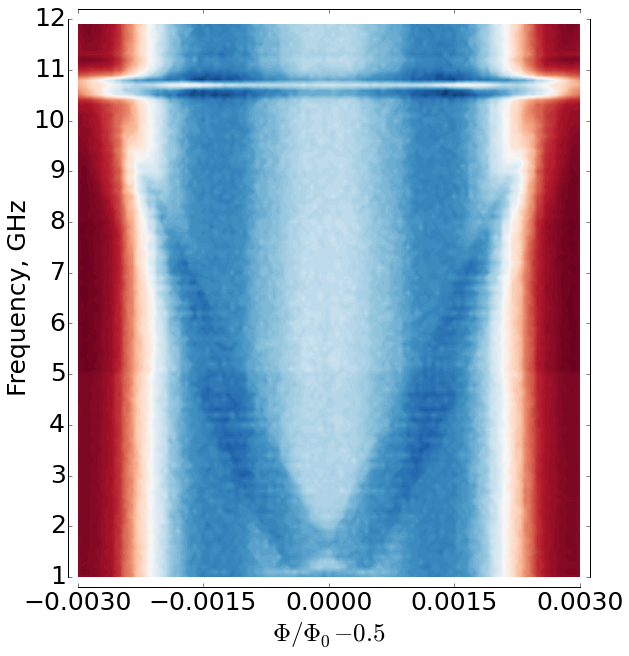
\includegraphics[valign=t, scale=.75]{Pictures/two-tone_spectrum3_pha} &
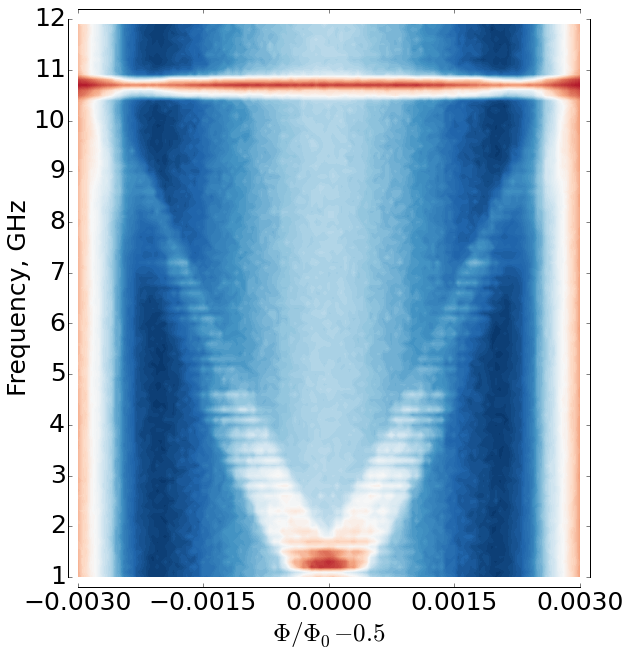
\includegraphics[valign=t, scale=.75]{Pictures/two-tone_spectrum3}\\
\parbox[bottom][.2cm][t]{10cm}{\captionof{subfigure}{$20\log|S_{21}|$ plot}} &
\parbox[bottom][.2cm][t]{10cm}{\captionof{subfigure}{$\text{Arg}\,[S_{21}]$ plot}} \\
\end{tabular}
\captionof{figure}{Two tone spectra}
\label{fig:two-tone}
\end{minipage}

\end{tcolorbox}

\columnbreak
%%%Column 2

\tcbset{colframe=titlecol}
\begin{tcolorbox}[left=1cm, right=1cm, top=0.5cm, bottom=0.5cm, 
                  title={\Large Rabi model}, bottomtitle=.5cm, toptitle=.5cm
                  ]
                  
The theoretical model describing the interaction of the qubit includes unitary dynamics governed by Rabi Hamiltonian, three channels of dissipation, microwave driving of resonator and taking the voltage drop proportional to $|\!\left< \hat a \right>\!|$ in the steady-state, where $\hat a$ is resonator destruction operator. The master equation to determine the latter follows:
\begin{equation}
\begin{gathered}
\mathcal{\hat H}_R = \frac{\hbar \omega_q}{2} \hat \sigma_z  + \hbar \omega_r  \left(\frac{1}{2}+\hat a^\dag \hat a \right) + \hbar g (\hat a^\dag + \hat a) \otimes \left( \hat \sigma_x \cos\theta-  \hat\sigma_z \sin\theta \right) +
 \\
 + A\cos(\omega t) (\hat a^\dag + \hat a) + \kappa \mathcal{D}[\hat a] + \gamma \mathcal{D}[\hat \sigma^-] + \gamma_\phi \mathcal{D}[\hat \sigma_z],
\end{gathered}
\end{equation}
where $\tan \theta = \frac{\Delta}{\varepsilon}$ and (1) and (2) were used to make right basis transformation. The spectrum including only $\omega_{01}$ and $\omega_{02}$ frequencies is shown on \autoref{fig:Rabi_spec}.\\

\begin{minipage}{\textwidth}
\centering
\begin{tabular}{c@{\hspace{1cm}}c}
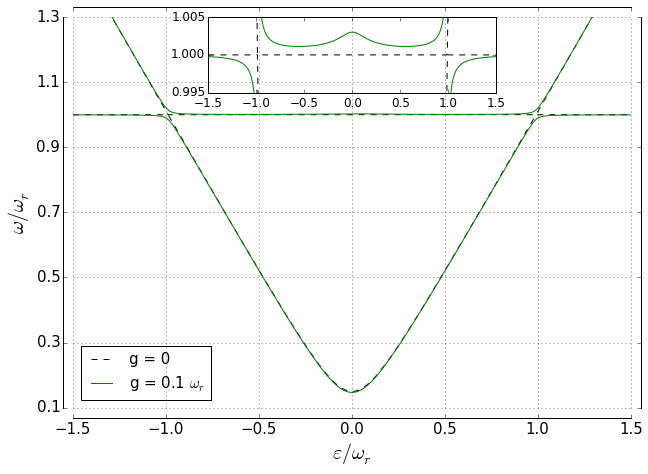
\includegraphics[valign=t, scale=0.8]{Pictures/Rabi_anticrossing_far} &
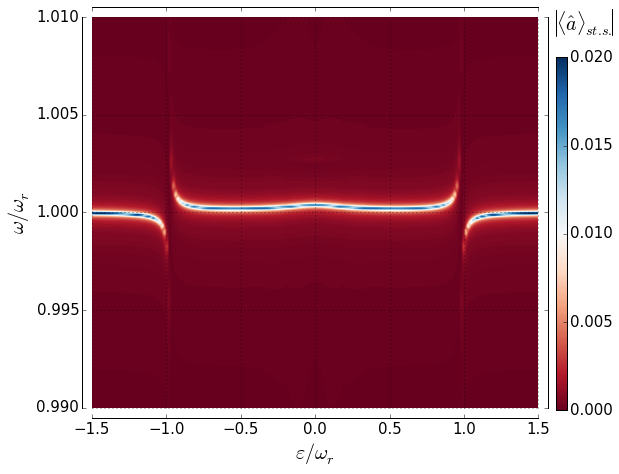
\includegraphics[valign=t, scale=0.8]{Pictures/Rabi_anticrossing_far_dyn}\\
\parbox[bottom][3cm][t]{16cm}{\captionof{subfigure}{Rabi anticrossings (stationary solution). Inset shows zoomed area around $\omega_r$ and reveals a feature of upper branch at the symmetry point.}} &
\parbox[bottom][3cm][t]{16cm}{\captionof{subfigure}{Spectrum obtained by numerical simulation with QuTiP\cite{johansson2012}. Parameters used: $\kappa = 5\cdot 10^{-4}$, $\gamma = 0.01,\ \gamma_\phi = 0.007,\ \Delta = 0.2\,\omega_r,\ g=0.03\,\omega_r$}}\\
\end{tabular}
\end{minipage}

\begin{minipage}{\textwidth}
\centering
\captionof{figure}{The static and dynamic spectra of Rabi Hamitlonian.}
\label{fig:Rabi_spec}
\end{minipage}

\begin{minipage}{\textwidth}
\begin{tabular}{l@{\hspace{1cm}}l}
\parbox{0.5\textwidth}{It can be seen on \autoref{fig:Rabi_spec}~(a) that at the degeneracy point both the frequencies have stronger deviations from unperturbed spectrum than in the other areas of dispersive regime. That happens due to the effective dependence of coupling constant $g_{eff} = g\cos\theta$ on flux.}
&
\parbox{0.45\textwidth}{\autoref{fig:Rabi_spec}~(b) shows how the system will react to driving with $A (\hat a^\dag + \hat a)\cos\omega t$. The part of the spectrum around $\omega_r$ will only be observed -- qubit flips are suppressed for this operator, so there is no absorption at the bare qubit frequency $\omega_q$.}\\
\end{tabular}
\end{minipage}
\end{tcolorbox}

\tcbset{colframe=titlecol}
\begin{tcolorbox}[left=1cm, right=1cm, top=0.5cm, bottom=0.5cm, 
                  title={\Large Anticrossings}, bottomtitle=.3cm,toptitle=.5cm
                  ]
\captionsetup[subfigure]{justification=centering}                  
                    
\begingroup
\setlength{\columnsep}{1cm}	
\begin{multicols}{2}
The main idea of the study was to compare the prediction of model (3) with the experimentally obtained spectrum. On \autoref{fig:anticrossing_double} the two outcomes are shown, theoretical (a) and experimental (b). The fitting parameters were the coupling constant, flux-axis scale, unknown bare resonator frequency and of course three dissipation rates. Although it is one of the best possible fits, there are significant differences between plots in the upper branch.  
\end{multicols}
\endgroup

\vspace{.5cm}
\begin{minipage}{\textwidth}

\hspace{-.5cm}
\begin{tabular}{c@{\hspace{0cm}}c}
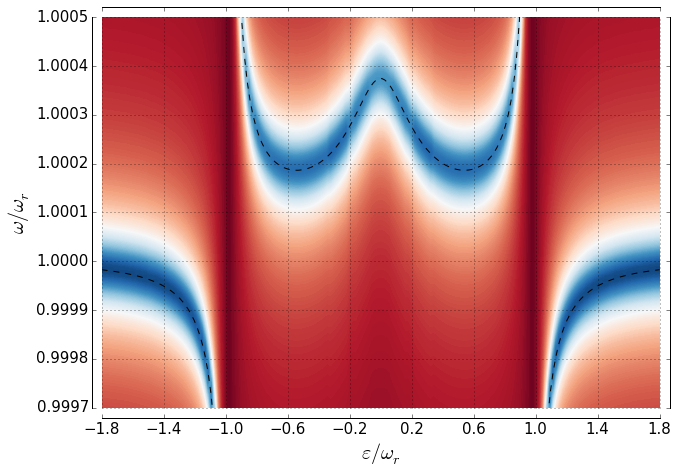
\includegraphics[valign=t, scale=.77]{Pictures/anticrossing_double1} &
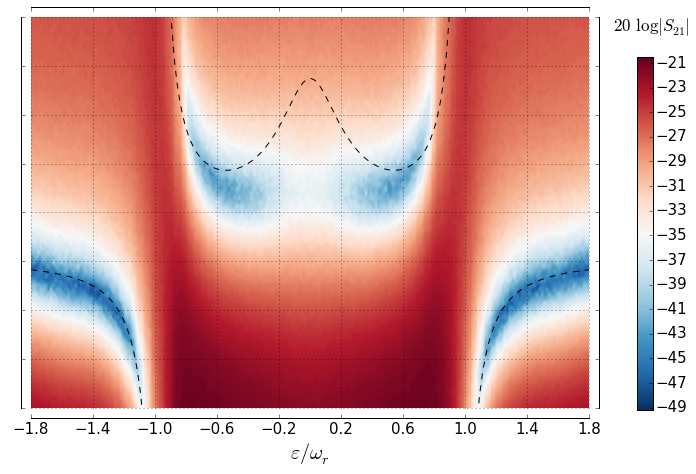
\includegraphics[valign=t, scale=.77]{Pictures/anticrossing_double2}\\
\parbox[bottom][2.5cm][t]{17cm}{\captionof{subfigure}{Theoretical plot (z-scale normalized). Parameters same as in \autoref{fig:Rabi_spec}~(b) except for increased $\kappa = 6.5 \cdot 10^{-4}$. Plot follows the dashed line.}} &
\parbox[bottom][2.5cm][t]{15cm}{\captionof{subfigure}{Experimental plot. The middle peak is absent and the upper branch is too low and too narrow. Lower branch matches.}} \\
\end{tabular}
\captionof{figure}{Theoretical vs. experimental data for anticrossings. The dashed line shows the prediction of stationary Schr\"{o}dinger equation to simplify comparison.}
\label{fig:anticrossing_double}
\end{minipage}

\vspace{1cm}
\begingroup
\setlength{\columnsep}{1cm}	
\begin{multicols}{2}
Another effect that was investigated was the ``vanishing of anticrossings''. That means the impossibility to observe Rabi splitting of absorption peak in resonant regime. In the limit of ``bad'' qubit (lifetimes up to 1000 times shorter than of the photon inside the resonator) it was possible to model this effect theoretically (qualitatively) - indeed, peaks fade out before entering the anticrossing area, see \autoref{fig:anticrossing_fade} and additionally \autoref{fig:Rabi_spec}~(b).
\end{multicols}
\endgroup

\vspace{.5cm}
\begin{minipage}{\textwidth}
\hspace{-.5cm}
\begin{tabular}{c@{\hspace{-0.3cm}}c}
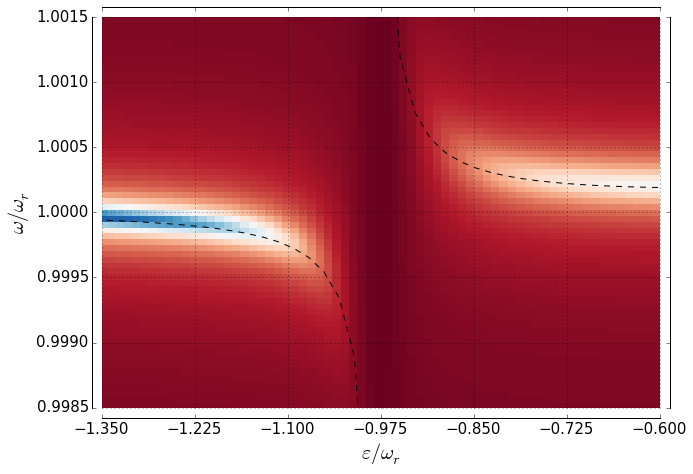
\includegraphics[valign=t, scale=.77]{Pictures/anticrossing_vanishing} &
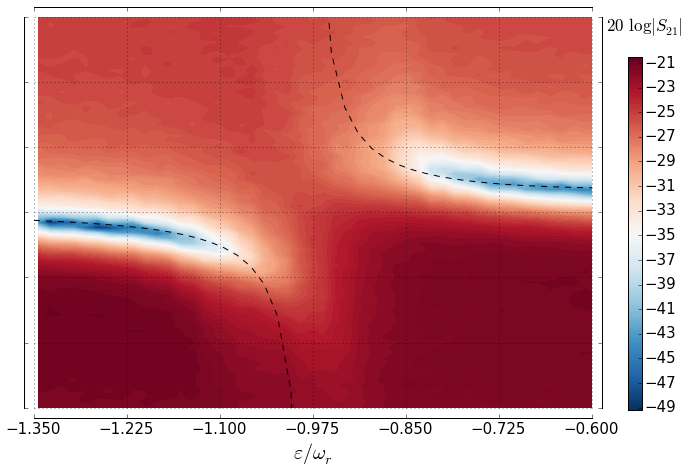
\includegraphics[valign=t, scale=.77]{Pictures/anticrossing_vanishing_exp}\\
\parbox[bottom][2.5cm][t]{17cm}{\captionof{subfigure}{Theoretical plot (z-scale normalized). Parameters same as in \autoref{fig:anticrossing_double}~(a) except for $\gamma = \gamma_\phi = 0.1$. Plot still follows the dashed line.}} &
\parbox[bottom][2.5cm][t]{15cm}{\captionof{subfigure}{Experimental plot. It can be seen that the right branch is much brighter than theory predicts and is too high above the dashed line.}} \\
\end{tabular}
\captionof{figure}{Theoretical vs. experimental data for anticrossing vanishing. The dashed line shows the prediction of stationary Schr\"{o}dinger equation to simplify comparison.}
\label{fig:anticrossing_fade}
\end{minipage}


\end{tcolorbox}

\tcbset{colframe=titlecol}
\begin{tcolorbox}[left=1cm, right=1cm, top=0.5cm, bottom=0.5cm, 
                  title={\Large Conclusion}, bottomtitle=.5cm,toptitle=.5cm
                  ]

The experiment we have conducted has shown that the our qubit-resonator system can't be described by Rabi model. This result must have its roots in the sample defects, which are nearly impossible to model. Nevertheless, qualitative effects are observable even with a bad qubit.

\end{tcolorbox}

\end{multicols}

\tcbset{colframe=titlecol}
\begin{tcolorbox}[left=1cm, right=1cm, top=0.5cm, bottom=0.5cm, 
                  title={\Large References}, bottomtitle=.5cm,toptitle=.5cm
                  ]
\begingroup
\renewcommand{\section}[2]{}%
\bibliographystyle{plain}
{\small
\bibliography{poster.bib}
}
\endgroup
\end{tcolorbox}
\end{document}
